
\section{Functional Electrical Stimulation}
\label{sec:FES}
\subsection{Overview}

Exercise and loading the leg bones can prevent the primary cause of these health side effects. Functional Electrical Stimulation (FES) is a rehabilitation tool used to stimulate muscle activation  \cite{quintero2012preliminary}. There are several benefits of using FES for SCI rehabilitation; clinical outcomes, fitness benefits, and functional gains \cite{hamid2008role}. FES has been used to allow people to stand, walk, and use a cycle\cite{mazzoleni2013fes}. All of which have measurable rehabilitation and health benefits. FES's main complication and limitation is muscle fatigue \cite{karu1995reducing}. Using FES  does not provide any structural support to hold up the person. FES can be supplemented by using mechanical structures to support the patient and add a layer of safety. 

\subsection{Muscle Modeling}
 In \cite{reiner1998patient}, simulation is used to model a patient-driven approach in which the the upper-body effort is used to stimulate leg muscles through Functional Electrical Stimulus (FES) \cite{lynch2008functional} \cite{rushton1997functional}. 
 
 \autoref{eq:activation} shows the muscle stimulation activation where, $a_r(t)$ is the activation based on the stimulation pulse width and $a_f(t)$ is the activation based on the stimulation frequency. The $fit(t)$ term controls the muscle fatigue which is a results of the calcium dynamics and shown in \autoref{eq:fatigue}. Here $\beta$ is a scaling term and, $T_{rec}$ and $T_{fat}$ are time constant terms that control how quickly the muscle recover and fatigue. This values are dependant on each of the muscles groups and need to be tuned the person. \autoref{fig:fagigueExample} shows an example of the effect of fatigue on the activation function, the blue line is the non-fatigued activation, the pulse value is being controlled over time. The orange line fatigued activation value as shown the maximum value is decreased. 
 
 
 
 \begin{equation}
     a &= fit(t) a_r(t) a_f(t)
     \label{eq:activation}
 \end{equation}
 
 \begin{equation}
    \small
    \begin{aligned}
             \frac{dfit}{dt} &= \frac{ (fit_{min} - fit) a \lambda(f) } {T_{fat} } + \frac{ (1 - fit) ( 1- a \lambda(f)) } {T_{rec} } \\
             \lambda(f) &= 1 - \beta + \beta(\frac{f}{100})^2 
    \end{aligned}
     \label{eq:fatigue}
 \end{equation}
 
 

 \begin{figure}
     \centering
     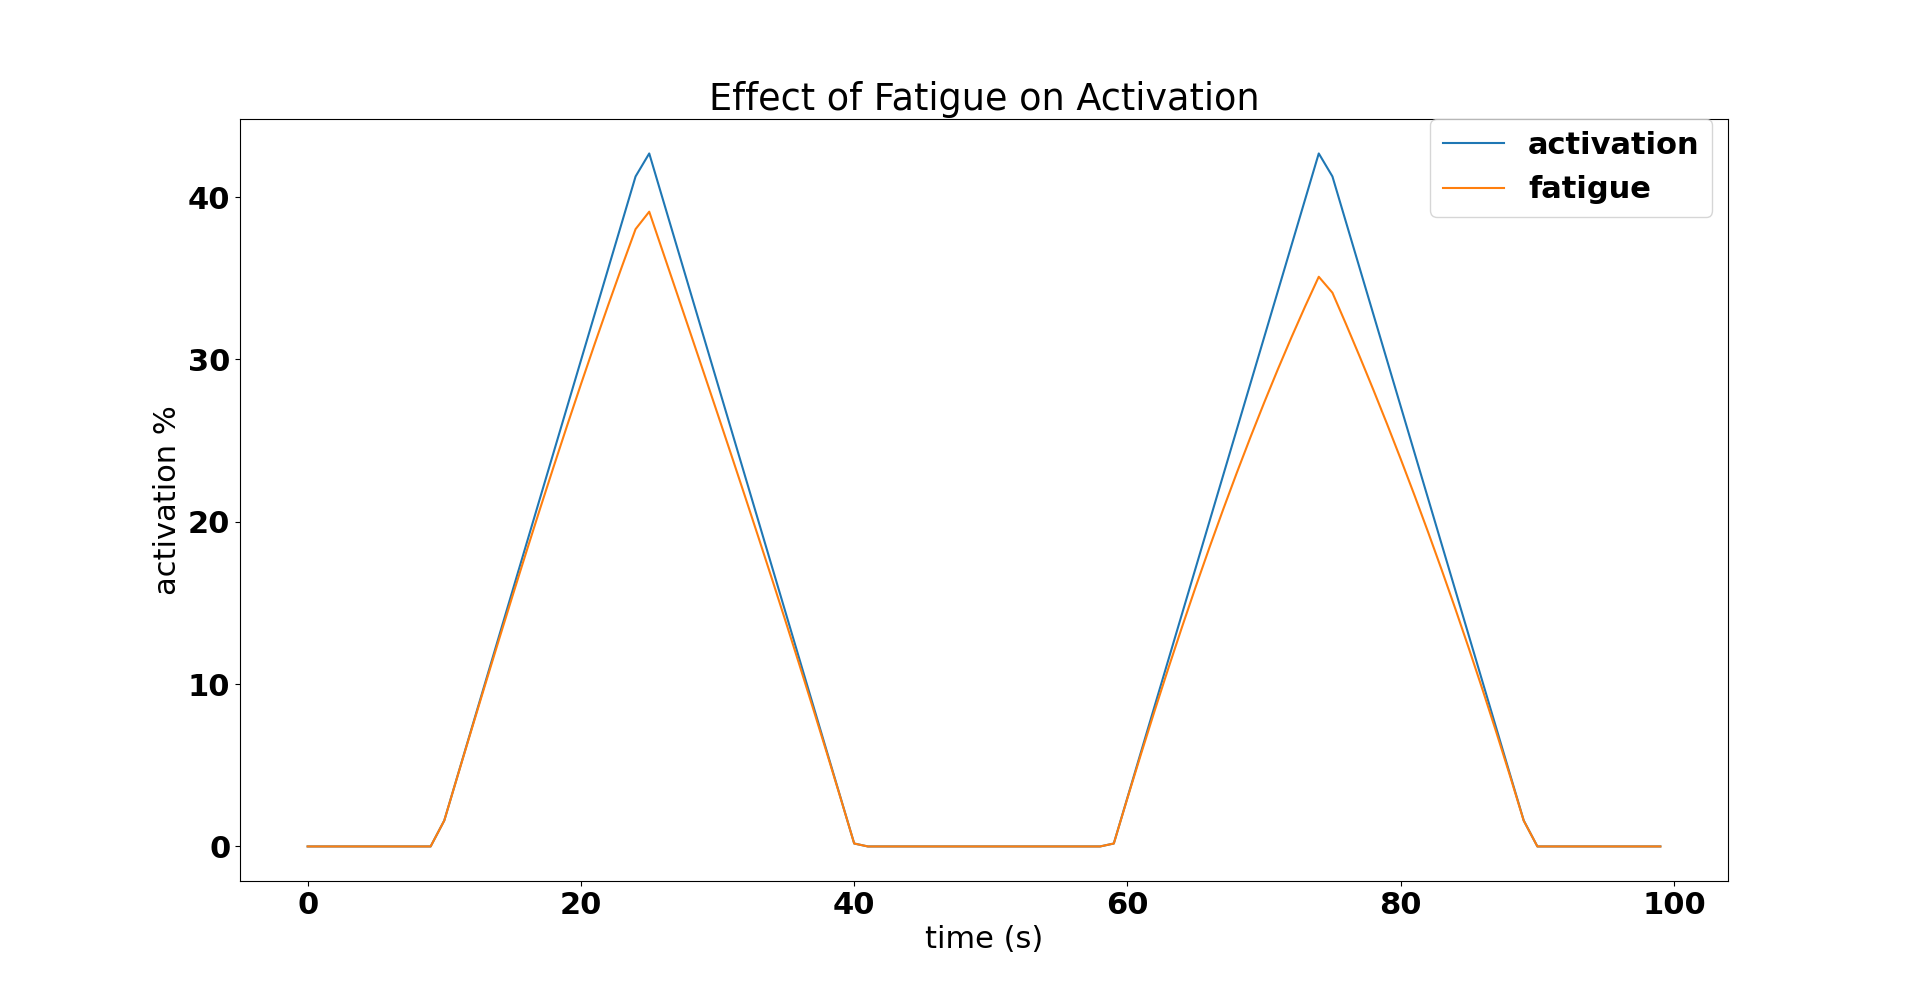
\includegraphics[width=\textwidth]{images/background/activation.png}
     \caption[Fatigue Example]{Fatigue Example}
     \label{fig:fagigueExample}
 \end{figure}
 
 
 The total torque is shown in \autoref{eq:totalMucsle}. The $M_{ela}$ term is calculated from the elastic properties of the muscles. The $M_{vis}$ term is calculated from the viscous properties of the muscles. The $M_{act}$ term is torque generated from the activation of muscles. These terms are dependant on the moment arms of each of the nine muscles groups in the lower body. This equations are non-linear terms that parameterized by the joint angles of the leg.  The $M_{dyn}$ are the dynamics of the model. 
 
 
 \begin{equation}
     \tau = M_{act} + M_{dyn} + M_{vis} + M_{ela}
     \caption{Total muscle force}
     \label{eq:totalMucsle}
 \end{equation}
 
